\chapter{Baselines}

\section{LSTM}


The LSTM baseline was implemented as a local sequence-to-one forecasting model trained independently for each selected item--store time series. In contrast to global forecasting models, which learn shared parameters across multiple products, this baseline model focuses on the temporal dynamics of a single product at a time. This makes it a suitable reference model for evaluating whether the proposed graph-based approaches provide additional value beyond the information contained in the target product’s historical demand and engineered covariates.

For each product--store pair, the original demand series is first divided into training, validation, and test segments. The target variable was scaled using a min-max transformation fitted only on the training segment, and the same fitted scaler was then applied to the validation and test periods. The same logic was applied to the exogenous variables, ensuring that information from the validation or test periods was not used to fit the preprocessing transformations.

The model receives a fixed-length input window of the past observations. Each training sample consists of a sequence of length \(L\), where each time step contains the historical target value and, when available, a vector of the exogenous variables. In the implemented dataset, the target sequence is defined as
\[
(y_{t-L}, y_{t-L+1}, \ldots, y_{t-1}),
\]
where the prediction target is the next value \(y_t\). When exogenous variables are used, they are concatenated with the target sequence at each time step, producing an input tensor of shape
\[
(\text{batch size}, L, 1 + p),
\]
where \(p\) is the number of exogenous features. This means that the LSTM receives both autoregressive information from the product’s past demand and deterministic or pre-computed calendar-related covariates. In the code, this sequence construction is handled by the custom \texttt{TimeSeriesDataset}, which stacks the target sequence with the corresponding exogenous feature sequence before returning the input--target pair.

The neural architecture is intentionally simple. It consists of one recurrent LSTM block, followed by a dropout layer and a fully connected linear output layer. The LSTM processes the input sequence in chronological order and produces a hidden representation for each time step. Only the hidden representation associated with the final time step is retained because the task is a one-step-ahead forecast. This final representation is passed through dropout and then through a linear layer that maps the hidden state to a single-scalar demand prediction:
\[
\hat{y}_t = W h_{t-1}^{(LSTM)} + b.
\]
Therefore, the implemented model follows the structure:
\[
\text{Input sequence} \rightarrow \text{LSTM} \rightarrow \text{last hidden state} \rightarrow \text{Dropout (if positive} \rightarrow \text{Linear layer} \rightarrow \hat{y}_t.
\]
This architecture is implemented in the \texttt{LSTM} class, where the recurrent layer uses \texttt{batch\_first=True}, the last LSTM output is selected, and a final linear layer produces a one-dimensional forecast.

Although the model is trained as a one-step-ahead predictor, it is used recursively during the test phase to generate a multi-step forecast over the entire forecasting horizon. The recursive procedure starts from the last available validation window, predicts the next demand value, appends this prediction to the input history, and then uses the updated sequence to predict the subsequent period. This process is repeated until all the test-period forecasts are generated. Therefore, after the first forecast step, the model gradually conditions its own previous predictions rather than only on the observed demand values. This recursive inference mechanism is implemented in the inference routine, where each predicted value is fed back into the rolling input sequence for subsequent predictions. :contentReference[oaicite:2]{index=2}

Therefore, the architecture can be interpreted as an autoregressive LSTM with exogenous inputs. Its main purpose in this dissertation is to provide a strong sequential baseline: it can model nonlinear temporal dependencies in the target series, incorporate calendar and holiday effects, and generate multi-step forecasts through recursive simulations. However, it does not explicitly use the relational information between products. Consequently, any improvement obtained by graph-based models can be interpreted as evidence that inter-product similarity or dependency structures provide useful information beyond the target product’s temporal history and engineered covariates.

\begin{figure}[h!]
    \centering
    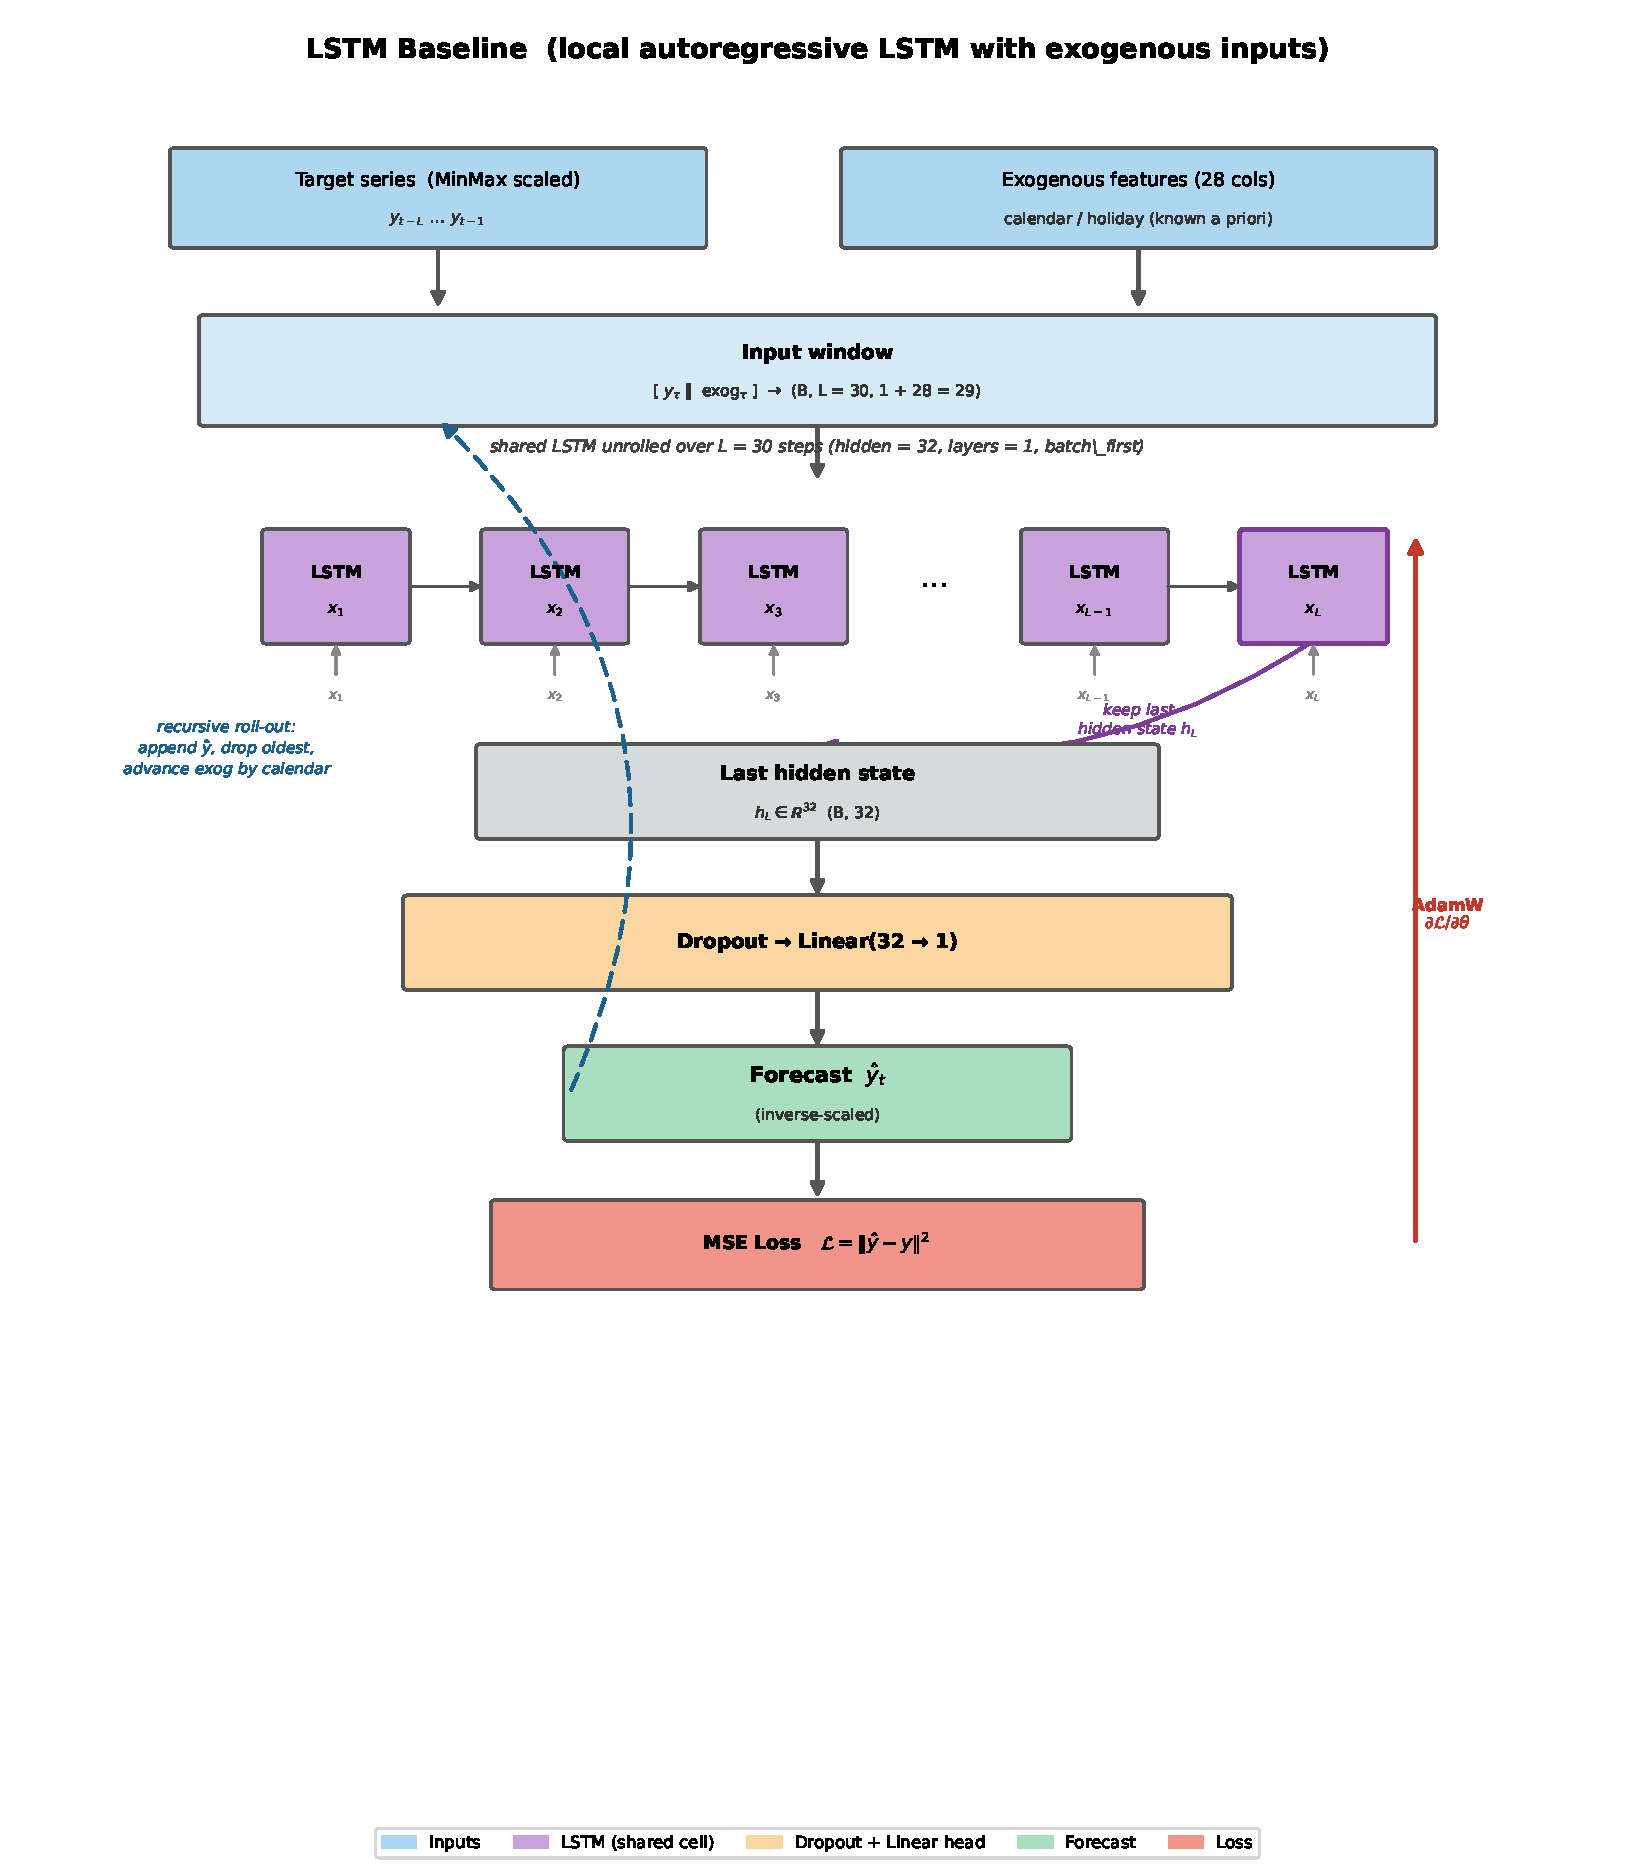
\includegraphics[width=1\linewidth]{figures/lstm_baseline_architecture.pdf}
    \caption{Local autoregressive LSTM with exogenous inputs. The MinMax-scaled target series and 28 calendar/holiday features were concatenated into an input window of length \(L=30\) and fed step-by-step through a shared single-layer LSTM (hidden size 32). The final hidden state \(\mathbf{h}_L\in\mathbb{R}^{B\times 32}\) is passed through a Dropout + Linear head to produce a one-step-ahead forecast \(\hat{y}_t\), trained end-to-end with MSE loss via AdamW. Multi-step forecasts are generated via recursive roll-out, appending each prediction as the next autoregressive input while advancing exogenous features by calendar.}
    \label{fig:placeholder}
\end{figure}
\subsection{Hyperparameters Chosen}
\label{subsec:lstm_hyperparameters_chosen}

The LSTM baseline was configured using a fixed set of architectural and optimization hyperparameters. Because the purpose of this model is to serve as a controlled sequential benchmark, the chosen configuration favors a relatively simple architecture, limiting the model capacity while still allowing the network to capture short-term nonlinear temporal dependencies in the demand series.

The input sequence length, or lookback window, was set to $L=30$. Therefore, each prediction was based on the previous 30 time steps of the target series and the corresponding exogenous variables. This choice provides the model access to approximately one month of recent demand history, capturing monthly cycles, payday effects, and weekly repeating patterns that are highly prevalent in retail data. The resulting input dimensionality is given by $d_{\text{input}} = 1 + p$, where the first component corresponds to the lagged target demand and $p$ is the number of exogenous features included in the model.

The final baseline architecture used one LSTM layer with 32 hidden units. A single recurrent layer was selected to maintain the baseline compact and reduce the risk of overfitting, especially because the model is trained locally for each item--store series rather than globally across all products. A hidden size of 32 provides a moderate latent representation capacity while keeping the number of trainable parameters relatively small. Dropout was set to 0.0. Because only one LSTM layer is used, the recurrent dropout between stacked LSTM layers is not active in the PyTorch implementation; therefore, disabling dropout also keeps the architecture deterministic and easier to interpret.

The model was trained using mini-batches of size 32 and optimized using the AdamW optimizer. The learning rate was fixed at $10^{-3}$, which is a commonly used initial value for Adam-based optimizers and provides a stable compromise between the convergence speed and training stability. The maximum number of epochs was set to 1000; however, the effective number of training epochs was controlled by early stopping with a patience of 100 epochs and validation-based model selection. This means that a large epoch budget acts as an upper bound rather than forcing the model to train for all epochs.

The loss function used during training and validation was the mean squared error (MSE). This choice is consistent with the objective of penalizing larger forecasting errors more strongly, which is relevant in a retail forecasting setting, where large deviations from the true demand have a severe operational and financial impact. In addition, a learning-rate scheduler was used to reduce the learning rate by half when the validation loss stopped improving, thereby allowing the optimizer to refine the solution after the initial training phase.

The selected LSTM hyperparameters are listed in Table \ref{tab:lstm_hyperparameters}.

\begin{table}[H]
\centering
\caption{Base LSTM hyperparameter configuration.}
\label{tab:lstm_hyperparameters}
\begin{tabular}{ll}
\hline
\textbf{Hyperparameter} & \textbf{Chosen value} \\
\hline
Lookback window ($L$) & 30 observations \\
Batch size & 32 \\
Hidden size & 32 \\
Number of LSTM layers & 1 \\
Dropout & 0.0 \\
Optimizer & AdamW \\
Learning rate & 0.001 \\
Maximum epochs & 1000 \\
Early stopping patience & 100 epochs \\
Loss function & MSELoss \\
\hline
\end{tabular}
\end{table}

This configuration defines a local autoregressive LSTM with an exogenous input. Its role is not to exhaustively maximize predictive performance through extensive hyperparameter tuning but rather to provide a transparent and reproducible neural baseline against which the proposed graph-based forecasting approaches can be compared.



\subsection{Feature Engineering}
\label{subsec:lstm_feature_engineering}

The LSTM baseline was trained using both historical target demand and a set of engineered exogenous variables. The objective of this feature engineering step is to provide the model with contextual information that may explain systematic variations in demand that are not fully captured by the raw autoregressive sequence alone. In particular, the selected features aim to represent short-term temporal dependence, weekly and monthly calendar effects, and demand changes around relevant holidays and special dates.

For each item--store series, the input at each time step is composed of the scaled target value and the corresponding exogenous feature vector. Therefore, the model input dimensionality is defined as
\[
d_{\text{input}} = 1 + p,
\]
where the first component corresponds to the historical demand value, and \(p\) denotes the number of exogenous variables. In the implemented configuration, the exogenous variables were generated before model training and then split into training, validation, and test segments consistent with the target series. The exogenous scaler is fitted only during the training period and then applied to the validation and test periods, avoiding the use of future information in the preprocessing stage.

The selected features were grouped into four main categories. The first group consists of basic calendar-position variables, namely, \texttt{day\_of\_week}, \texttt{day\_of\_month}, \texttt{week\_of\_year}, \texttt{week\_of\_month}, \texttt{month}, and \texttt{quarter}. These variables provide the model with information about the position of each observation within the weekly, monthly, quarterly, and annual cycles. This is particularly relevant in retail demand forecasting, as customer behavior may vary systematically across weekdays, month boundaries, and seasonal periods.

The second group contains binary calendar indicators, such as \texttt{is\_weekend}, \texttt{is\_monday}, \texttt{is\_friday}, \texttt{is\_month\_start}, \texttt{is\_month\_end}, \texttt{is\_quarter\_start}, and \texttt{is\_quarter\_end}. These features allow the model to identify specific positions in the calendar that may be associated with recurring demand. For example, weekends may reflect different shopping patterns from weekdays, whereas the beginning or end of a month may capture changes associated with salary cycles, household restocking, or operational planning periods.

The final group represents holiday- and event-related effects. This includes general holiday indicators such as \texttt{is\_holiday}, specific events such as \texttt{is\_thanksgiving}, \texttt{is\_black\_friday}, \texttt{is\_christmas}, \texttt{is\_christmas\_eve}, and \texttt{is\_new\_year\_eve}, and pre- and post-holiday proximity indicators.
\[
\texttt{is\_pre\_holiday\_1},\ 
\texttt{is\_pre\_holiday\_2},\ 
\texttt{is\_pre\_holiday\_3},\ 
\texttt{is\_pre\_holiday\_7},
\]
\[
\texttt{is\_post\_holiday\_1},\ 
\texttt{is\_post\_holiday\_2},\ 
\texttt{is\_post\_holiday\_3},\ 
\texttt{is\_post\_holiday\_7}.
\]
These variables are included because retail demand is often affected not only by the holiday itself but also by the days immediately before and after it. For instance, demand may increase before major holidays owing to stockpiling behavior and decrease afterwards owing to temporary saturation. The \texttt{is\_bridge\_day} feature further captures days between holidays and weekends, which may also alter regular purchasing behavior.

Therefore, the final feature set was designed to balance explanatory richness and parsimony. It includes variables that are either known in advance from the calendar or can be constructed from previously observed demand. Rolling mean features were considered but excluded from the base configuration. This choice keeps the baseline simpler and avoids adding smoothed versions of the target that may overlap with the information already provided by the explicit lag variables and LSTM lookback window. In addition, excluding rolling averages reduces the risk of introducing ambiguity during recursive multi-step inference, in which future target-dependent features must be updated using previous predictions rather than observed values.

During recursive inference, lag-based features require special treatment because future lags are not directly observed. After each prediction, the forecasted value was appended to the demand history and used to update the lag-based exogenous variables for subsequent steps. This ensures that the multistep forecasting procedure remains consistent with the recursive nature of the LSTM baseline: once the test horizon begins, the model progressively relies on its previous predictions when constructing future autoregressive inputs.

Overall, the engineered features make the LSTM baseline more informative than a purely univariate, recurrent model. The baseline remains local to each item--store series, but it is allowed to condition its forecasts on calendar structure, recent demand memory, and holiday-related demand effects. This provides a stronger and fairer benchmark for evaluating whether graph-based models add predictive value beyond temporal and calendar-driven information.


\section{Time-Distributed MLP}

The time-distributed multilayer perceptron (TimeDistributedMLP) baseline is implemented as a feed-forward forecasting model that maps a fixed historical input window into a one-step-ahead demand prediction. Similar to the LSTM baseline, the model is trained locally for each item--store series and uses the same type of input information: past target demand values and, when available, engineered exogenous variables. However, unlike LSTM, the model does not contain recurrent connections, gates, or memory states. Instead, it processes each time step of the input window independently through a shared MLP encoder and aggregates the resulting hidden representations.

Let \(L\) denote the lookback window length and \(C\) denote the number of input channels at each time step. In this setting,
\[
C = 1 + p,
\]
where the first channel corresponds to the historical target demand, and \(p\) is the number of exogenous variables. Therefore, each input sample is represented as
\[
\mathbf{X}_t \in \mathbb{R}^{L \times C}.
\]

Rather than flattening the entire temporal window into a single vector of dimension \(L \cdot C\), the TimeDistributedMLP applies the same feedforward network to each time step:
\[
\mathbf{h}_{t-j} = f_{\theta}(\mathbf{x}_{t-j}), 
\qquad j = 1,\ldots,L,
\]
where \(\mathbf{x}_{t-j} \in \mathbb{R}^{C}\) is the feature vector associated with one time step, and \(f_{\theta}\) is a shared MLP encoder. This weight sharing implies that the same nonlinear transformation is applied across all positions in the lookback window.

Each hidden representation is computed using fully connected layers with nonlinear activation and dropout regularization:
\[
\mathbf{h}^{(1)}_{t-j} = \phi(W^{(1)}\mathbf{x}_{t-j} + b^{(1)}),
\]
\[
\mathbf{h}^{(l)}_{t-j} = \phi(W^{(l)}\mathbf{h}^{(l-1)}_{t-j} + b^{(l)}).
\]

After all the time steps were encoded, the model summarized the temporal window using two complementary representations. The first is the hidden vector of the most recent time step,
\[
\mathbf{h}_{last} = \mathbf{h}_{t-1},
\]
which preserves information from the most recently observed demand state. The second is the mean-pooled representation over the full lookback window,
\[
\bar{\mathbf{h}} = \frac{1}{L}\sum_{j=1}^{L}\mathbf{h}_{t-j},
\]
This provides a global summary of the recent historical context.

These two vectors were concatenated.
\[
\mathbf{c}_t = [\mathbf{h}_{last} \, || \, \bar{\mathbf{h}}],
\]
and passed through a final linear layer to obtain a one-step-ahead forecast:
\[
\hat{y}_{t} = W_o \mathbf{c}_t + b_o.
\]

In the implemented architecture, the model outputs a tensor of the following shape:
\[
\hat{\mathbf{Y}}_t \in \mathbb{R}^{1 \times 1},
\]
corresponding to a single-step prediction of the target demand variable. Therefore, forecasts over longer horizons are produced recursively: after each prediction, the input window is advanced by one step, and the predicted value is inserted into the history used for subsequent forecasts.

The overall architecture can be summarized as follows:
\[
\text{Input window }(L \times C)
\rightarrow
\text{shared timestep MLP}
\rightarrow
\text{last-step representation + mean pooling}
\rightarrow
\text{output layer}
\rightarrow
\text{one-step forecast}.
\]

This baseline provides a useful comparison with the LSTM because it tests whether nonlinear transformations of per-timestep demand and exogenous features, combined with a simple temporal aggregation mechanism, are sufficient for forecasting. While the LSTM learns sequential dependencies through recurrent hidden states, the TimeDistributedMLP relies on shared feed-forward encodings and a compact summary of the look-back window. Consequently, it remains simpler and faster to train than recurrent architectures while retaining some temporal information through the explicit use of the most recent hidden state and the average historical context. However, because it does not recursively model temporal transitions inside the network, it may be less capable of capturing complex ordered dependencies than an LSTM.


\subsection{Hyperparameters Chosen}
\label{subsec:mlp_hyperparameters_chosen}

The MLP baseline was configured as a feedforward neural forecasting model using a fixed training setup. The hidden structure consists of two fully connected layers with 128 and 64 neurons. This configuration provides the model with sufficient capacity to learn nonlinear relationships between the input window, engineered exogenous variables, and future demand horizon, while remaining simpler than recurrent or graph-based models. A dropout rate of 0.2 was applied to reduce overfitting and improve generalization.

The model was trained using mini-batches of 32 samples each. This batch size provides a compromise between stable gradient estimates and computational efficiency of the model. The learning rate was set to \(0.001\), and the maximum number of training epochs was set to 1000. This epoch value should be interpreted as an upper training budget, because training is controlled through validation performance and early stopping, with a patience value of 150 epochs.

The optimization was performed using AdamW with a weight decay of \(10^{-4}\). The inclusion of weight decay adds a small regularization effect by penalizing large parameter values, helping reduce overfitting while maintaining the flexibility of the neural model.

The loss function used for the main configuration was the mean squared error.
\[
    \mathcal{L}_{MSE} =
    \frac{1}{n}\sum_{i=1}^{n}(y_i - \hat{y}_i)^2.
\]
This objective penalizes larger forecasting errors more strongly, which is appropriate in the retail forecasting context, where large deviations may have a greater operational impact.

\begin{table}[H]
\centering
\caption{Base MLP hyperparameter configuration.}
\label{tab:mlp_hyperparameters}
\begin{tabular}{ll}
\hline
\textbf{Hyperparameter} & \textbf{Chosen value} \\
\hline
Batch size & 32 \\
Hidden layers & $(128, 64)$ \\
Activation function & ReLU \\
Dropout & 0.2 \\
Optimizer & AdamW \\
Learning rate & 0.001 \\
Weight decay & $10^{-4}$ \\
Maximum epochs & 1000 \\
Early stopping patience & 150 \\
Loss function & MSELoss \\
Lookback window & 30 \\
Forecast horizon & 153 \\
Validation size & 30 \\
\hline
\end{tabular}
\end{table}

Overall, the selected hyperparameters defined a controlled, nonlinear baseline. The goal was not to create an excessively complex model but rather to provide a reliable benchmark capable of learning from lagged target values and engineered exogenous variables before comparing them with recurrent and graph-based forecasting architectures.
\subsection{Feature Engineering}
\label{subsec:mlp_feature_engineering}

The MLP baseline was trained using the historical target demand and a set of engineered exogenous variables. The objective of this feature engineering step was to provide the model with explicit temporal and contextual information that may explain systematic variations in demand. This is particularly important for MLP because, unlike recurrent architectures, they do not maintain an internal hidden state over time. Instead, it receives information through a fixed input window and infers the temporal structure directly from the flattened input representation.

For each item--store series, the input sample was constructed from a fixed lookback window containing the scaled target values and the corresponding exogenous feature vectors. Therefore, if the lookback window has a length \(L\), the model input dimensionality is defined as
\[
d_{\text{input}} = L(1+p),
\]
where the first component at each time step corresponds to the historical demand value, and \(p\) denotes the number of exogenous variables. The exogenous variables were generated before model training and then split into training, validation, and test segments consistent with the target series. Any scaling applied to the exogenous variables was fitted only during the training period and then applied to the validation and test periods, avoiding the use of future information in the preprocessing stage.

The selected features were grouped into four main categories. The first group consists of cyclical calendar-position variables.
\[
\begin{split}
&\texttt{dow\_sin},\quad \texttt{dow\_cos},\\
&\texttt{doy\_sin},\quad \texttt{doy\_cos},\\
&\texttt{dom\_sin},\quad \texttt{dom\_cos},\\
&\texttt{wom\_sin},\quad \texttt{wom\_cos},\\
&\texttt{month\_sin},\quad \texttt{month\_cos},\\
&\texttt{quarter\_sin},\quad \texttt{quarter\_cos},\\
&\texttt{woy\_sin},\quad \texttt{woy\_cos}.
\end{split}
\]
These variables encode the position of each observation within the weekly, monthly, quarterly, and annual cycles. Sine and cosine transformations were used instead of simple ordinal values because they preserved the cyclical nature of time. For example, the transition from Sunday to Monday, December to January, or the last week of the year to the first week of the following year should be interpreted as a short temporal distance rather than a large numerical jump. By representing calendar positions using paired sine and cosine components, the MLP can learn smoother periodic patterns across multiple temporal cycles.

The second group contains binary calendar boundary indicators:
\[
\texttt{is\_month\_start},\quad
\texttt{is\_month\_end},\quad
\texttt{is\_quarter\_start},\quad
\texttt{is\_quarter\_end}.
\]
These features allow the model to identify specific positions in the calendar that may be associated with recurring demand. For example, the beginning or end of a month may capture changes related to purchasing behavior, replenishment routines, reporting cycles, salary effects, or other operational patterns. Similarly, quarterly boundaries may reflect changes associated with planning, inventory management, or business reporting periods.

The third group is composed of short-term demand-level features.
\[
\texttt{rolling\_mean\_excl\_7}.
\]
This variable provides a smoothed signal of recent demand intensity based on historical observations, excluding the current target value. As a result, it can be used during training without directly leaking the predicted value. This feature helps the MLP identify whether a product is currently in a higher- or lower-demand regime, complementing the raw lagged target values already included in the fixed input window. This is especially useful for a feed-forward model because it does not update a recurrent memory state as it processes the sequence.

The fourth group represents holiday- and event-related effects. This includes the general holiday indicator
\[
\texttt{is\_holiday},
\]
as well as specific retail-relevant events.
\[
\texttt{is\_thanksgiving},\quad
\texttt{is\_black\_friday},\quad
\texttt{is\_christmas},\quad
\texttt{is\_christmas\_eve},\quad
\texttt{is\_new\_year\_eve}.
\]
The feature
\[
\texttt{is\_bridge\_day}
\]
is also included to identify days between holidays and weekends. These variables were included because retail demand can change sharply on specific dates. Major holidays and shopping events may produce demand spikes, whereas bridge days may deviate from normal weekday behavior due to altered shopping routines, store visits, or household planning patterns.

Therefore, the final feature set was designed to provide the MLP with explicit information about the calendar position, structural calendar boundaries, recent demand intensity, and special retail events. Compared with the LSTM baseline, the MLP uses cyclical sine--cosine encodings more extensively because it does not process the input sequence through a recurrent hidden state. These encodings help the model interpret recurring temporal patterns from a flattened representation of the input window.

During recursive inference, target-dependent features require special treatment because future observed demand values are no longer available. In particular, the rolling mean feature must be updated using the available demand history, which progressively includes previous predictions once the test horizon begins. After each forecast, the predicted value was appended to the demand history and used to construct the input features for the subsequent steps. This ensures that the multistep forecasting procedure remains consistent with the recursive nature of the MLP baseline.


\section{Training Strategies and Model Selection}
\label{subsec:lstm_training_strategies}

The LSTM baseline was trained and evaluated using a chronological forecasting setup. For each item--store series, the available observations were divided into three consecutive segments: a training period, a validation period, and a final test period. The test period was kept completely unseen during training and model selection, and was only used for the final recursive forecasting evaluation. This setup preserves the temporal order of the demand series and avoids information leakage from future observations.
\begin{figure}[h!]
    \centering
    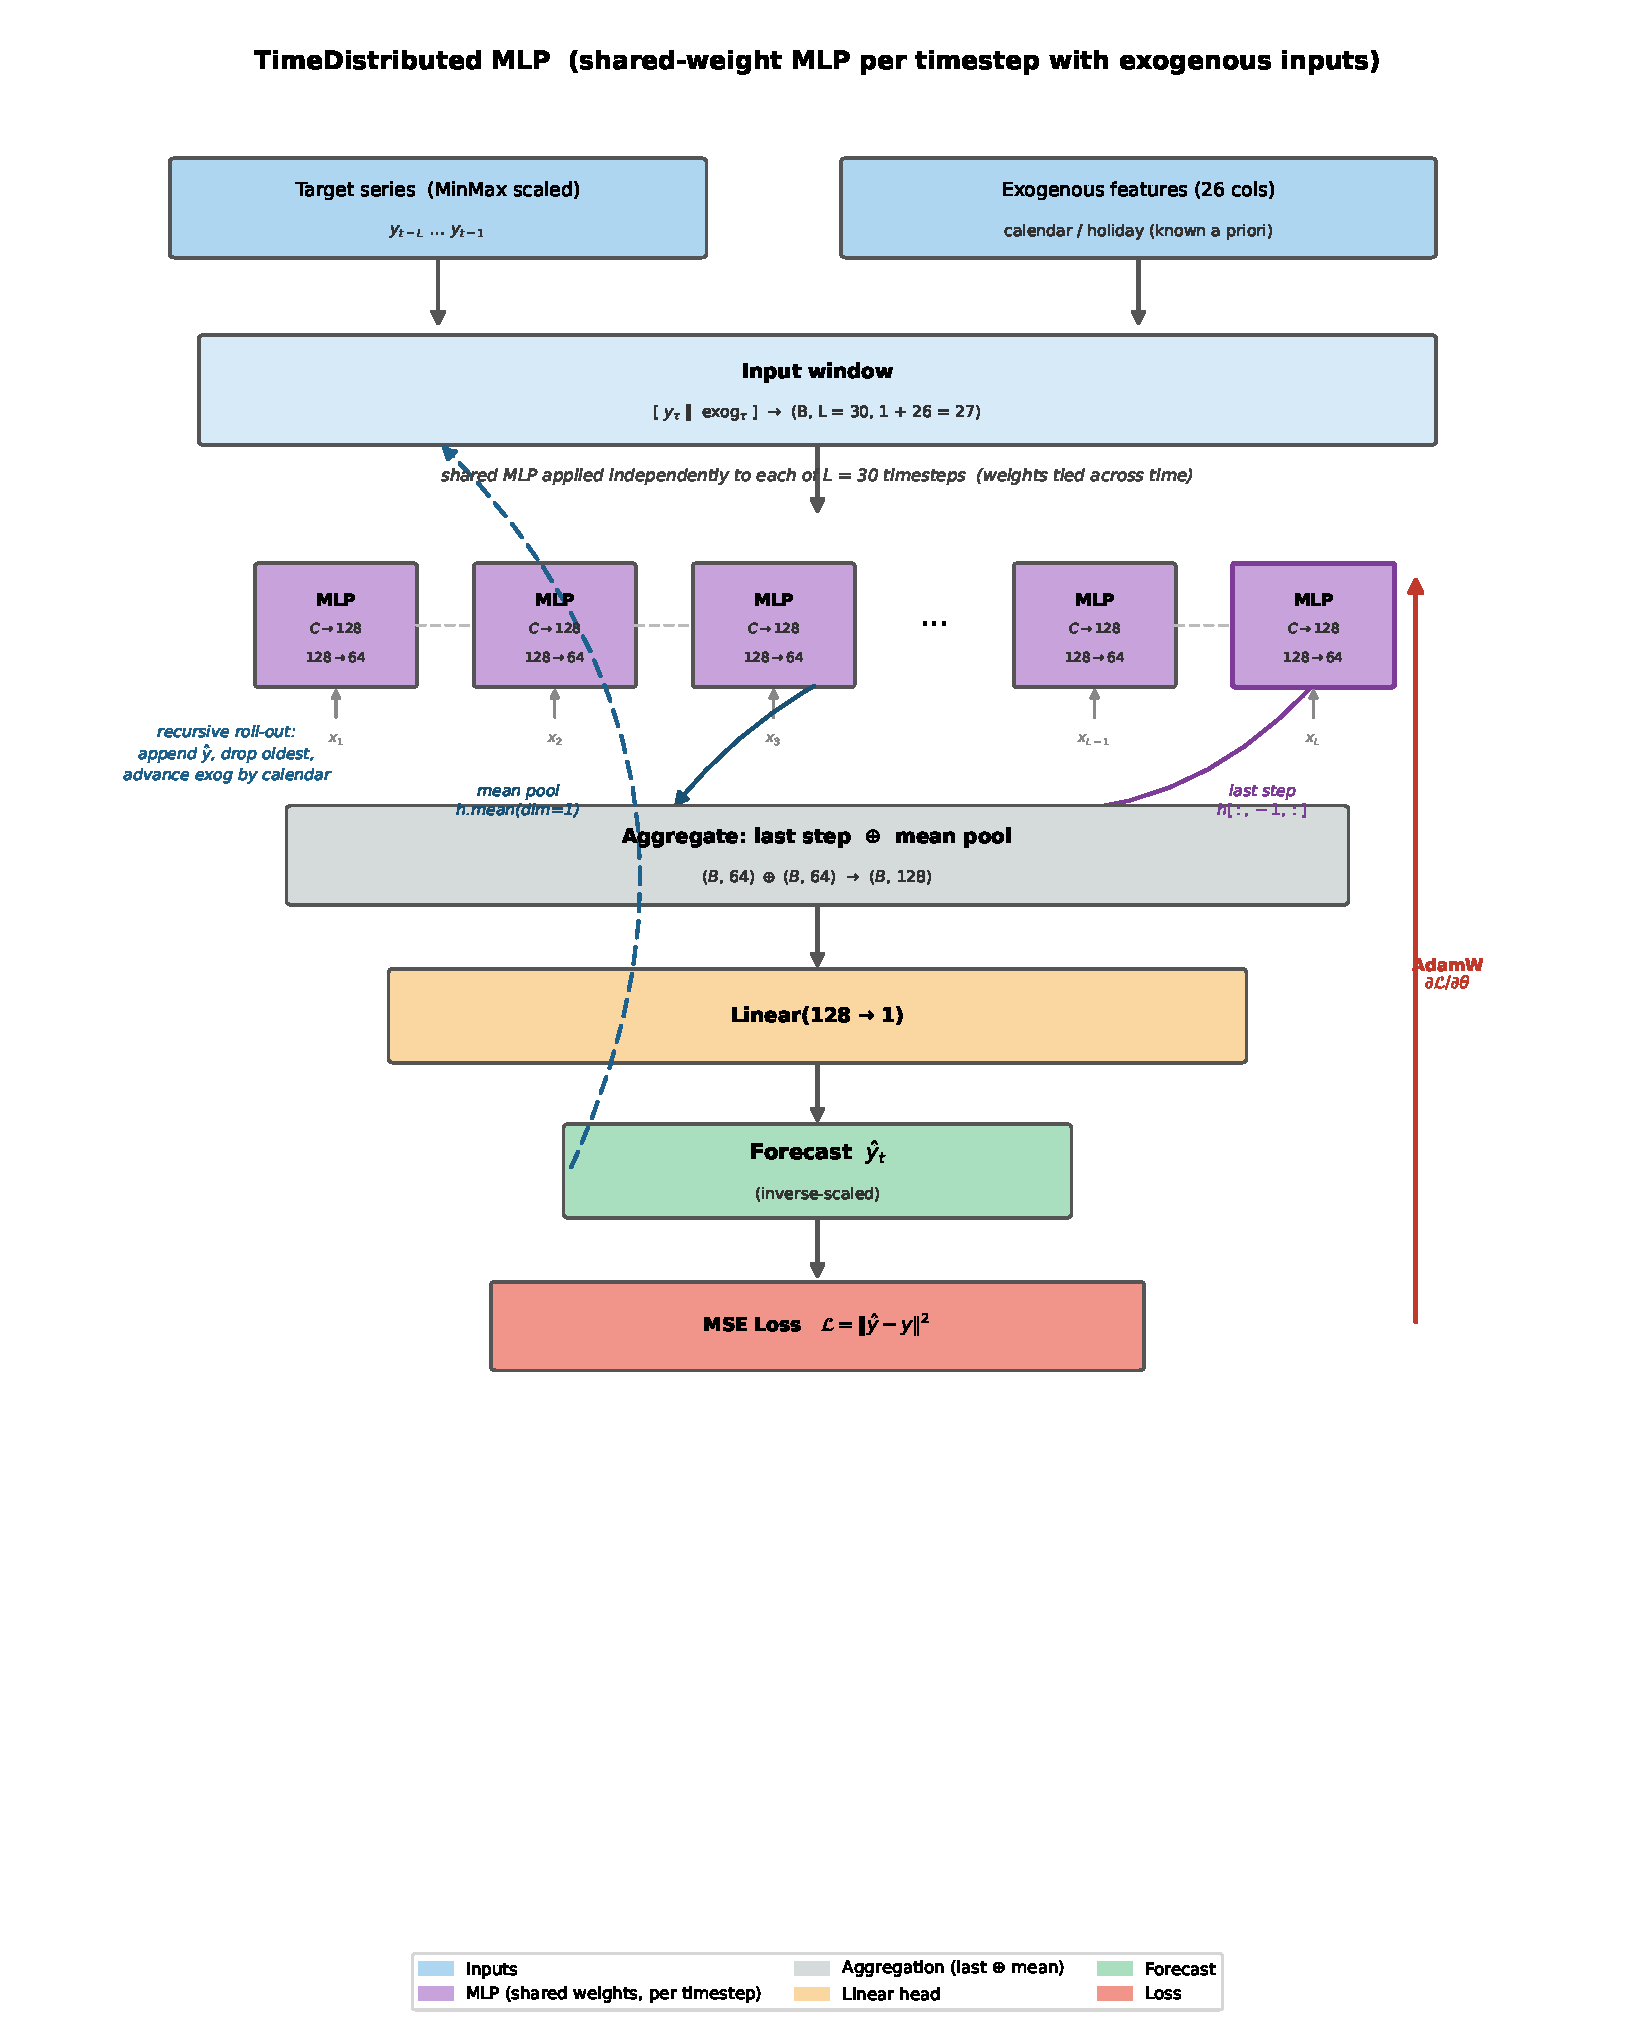
\includegraphics[width=1\linewidth]{figures/tdmlp_architecture.pdf}
    \caption{Local autoregressive MLP with exogenous inputs where weights are shared across time. At each step $\tau$, the concatenated input $[y_\tau \parallel \text{exog}_\tau] \in \mathbb{R}^{27}$ is passed through the same two-layer MLP ($C \to 128 \to 64$, ReLU + Dropout), producing a sequence of hidden representations $h \in \mathbb{R}^{B \times L \times 64}$. Two complementary signals are then extracted: the last step $h[:, -1, :]$ (recency) and the temporal mean $\bar{h}$ (global context), which are concatenated into $(B, 128)$ and projected by a single linear ($128 \to 1$) head to yield the one-step-ahead forecast $\hat{y}_t$. Training minimises MSE via AdamW; multi-step forecasts are generated by recursive roll-out, feeding each $\hat{y}_t$ back as the next autoregressive input while advancing the exogenous features by calendar.}
    \label{fig:placeholder}
\end{figure}

Before training, the target demand values were scaled using a Min--Max scaler fitted only on the training segment. The same fitted scaler was then applied to the validation segment. The exogenous variables were processed in the same way: the exogenous scaler was fitted on the training period and then used to transform the validation and test periods. After preprocessing, the training and validation datasets were converted into fixed-length input sequences using the selected lookback window. The data loaders were created without shuffling, preserving the temporal structure of the samples.

For each training strategy, a new LSTM model was initialized with the same architecture and optimization hyperparameters. The model was trained using the Adam optimizer and the mean squared error loss. A learning-rate scheduler was also used to reduce the learning rate when the validation loss reached a plateau, allowing the optimizer to continue refining the model after the initial learning phase. The maximum number of epochs was set to 1000, but the actual training duration was controlled by early stopping with a patience parameter. Therefore, the epoch budget acts as an upper bound rather than a fixed training length.

Several model selection strategies were considered in order to assess how sensitive the LSTM baseline is to the way the validation period is used. These strategies differ in how the final model checkpoint is selected and in how the training and validation observations are exploited.

\subsection{Best Validation Loss}

The first strategy corresponds to the standard validation-based model selection procedure. The model is trained on the training segment and evaluated on the validation segment after each epoch. Whenever the validation loss improves, the current model parameters are saved as the best checkpoint. Training stops when the validation loss does not improve for a predefined number of epochs.

This strategy selects the model that generalizes best to the validation period according to the MSE criterion:
\[
    \theta^{*} = \arg\min_{\theta_e} \mathcal{L}_{val}(\theta_e),
\]
where \(\theta_e\) denotes the model parameters after epoch \(e\), and \(\mathcal{L}_{val}\) is the validation loss. This is the most conventional strategy and provides a direct safeguard against overfitting the training segment.

\subsection{Best Training Loss with Validation-Based Early Stopping}

The second strategy separates the checkpoint selection criterion from the stopping criterion. In this case, the model checkpoint is saved whenever the training loss reaches a new minimum, while the validation loss is still monitored for early stopping. Therefore, the selected model corresponds to the lowest empirical training error, but the validation period continues to control how long the model is allowed to train.

This strategy can be written as:
\[
    \theta^{*} = \arg\min_{\theta_e} \mathcal{L}_{train}(\theta_e),
\]
while early stopping is triggered based on the evolution of \(\mathcal{L}_{val}\). This approach was included to test whether a model that fits the observed training demand more closely can produce better recursive forecasts, while still limiting excessive overfitting through validation-based stopping.

\subsection{Combined Training and Validation Retraining}

The third strategy uses the validation period to determine the optimal training duration and then exploits both the training and validation observations to fit the final model. First, the standard validation-loss strategy is applied to identify the best epoch. After that, the training and validation segments are concatenated and the model is further trained using the combined dataset.

The motivation for this strategy is that, once the number of training epochs has been selected using the validation period, the validation observations can be reused as additional historical data before forecasting the test horizon. This is particularly relevant in local item-level forecasting, where each model is trained on a relatively limited number of observations. By combining the training and validation periods, the final model has access to the most recent observed demand patterns before the test period begins.

However, this strategy no longer has an independent validation segment during the final training phase. As a result, it relies on the previously selected training duration to control overfitting. The validation period is therefore used for model selection, while the final model is fitted on all available pre-test observations.

\subsubsection{Expanding Window Training}

The fourth strategy follows an expanding-window procedure. Instead of using a single fixed training and validation split, the model is trained progressively across multiple temporal windows. The first window uses the initial training segment and validates on the immediately following block. Then, the training window is expanded by incorporating new observations, and the validation window moves forward. This process is repeated until the available pre-test period has been covered.

At window \(k\), the training set can be represented as:
\[
    \mathcal{T}_k = \{y_1, y_2, \ldots, y_{t_k}\},
\]
and the validation block as:
\[
    \mathcal{V}_k = \{y_{t_k+1}, \ldots, y_{t_k+h}\},
\]
where \(h\) is the validation step size. After each window, the training set grows:
\[
    \mathcal{T}_{k+1} \supset \mathcal{T}_k.
\]

This strategy simulates a realistic longitudinal forecasting scenario, where more observations become available over time and the model is repeatedly updated with an increasing historical record. The model weights are retained between windows, meaning that the model is fine-tuned progressively rather than reinitialized at each step. The final checkpoint is selected according to the lowest validation loss observed across all expanding windows.



\subsubsection{Sliding Window Training}

The fifth strategy follows a sliding-window procedure. In this case, the size of the training window remains fixed, but the window moves forward through time. At each step, the model is trained on a recent block of observations and validated on the immediately following block. Unlike the expanding-window strategy, older observations are discarded as the training window advances.

At window \(k\), the training set is defined as:
\[
    \mathcal{T}_k = \{y_{s_k}, y_{s_k+1}, \ldots, y_{t_k}\},
\]
and the next window becomes:
\[
    \mathcal{T}_{k+1} = \{y_{s_k+h}, y_{s_k+h+1}, \ldots, y_{t_k+h}\}.
\]
Thus, the window length remains constant, but both its start and end points move forward.



This strategy is particularly relevant for non-stationary retail demand, where older demand behaviour may become less representative of the current regime. By focusing on the most recent observations, the sliding-window approach gives more importance to recent patterns and reduces the influence of older periods that may reflect outdated seasonality, pricing, or customer behaviour. As in the expanding-window strategy, the model is fine-tuned across windows and the final checkpoint is selected based on the lowest validation loss observed across all windows.

\begin{table}[h!]
\centering
\caption{Summary of LSTM training and model selection strategies.}
\label{tab:lstm_training_strategies}
\begin{tabular}{lll}
\hline
\textbf{Strategy} & \textbf{Training data} & \textbf{Model selection criterion} \\
\hline
Best validation loss & Fixed training split & Lowest validation loss \\
Combined & Train + validation after epoch selection & Epoch selected using validation loss \\
Expanding window & Growing training window & Lowest validation loss across windows \\
Sliding window & Fixed-size moving training window & Lowest validation loss across windows \\
\hline
\end{tabular}
\end{table}

After training, the selected checkpoint for each strategy is loaded and evaluated on the test period using recursive multi-step inference. The model starts from the final validation window, predicts the next value, appends this prediction to the input history, and repeats the process until the full forecasting horizon is generated. This recursive procedure ensures that all strategies are evaluated under the same forecasting conditions.

\begin{figure}[h!]
    \centering
    \begin{subfigure}[t]{0.48\linewidth}
        \centering
        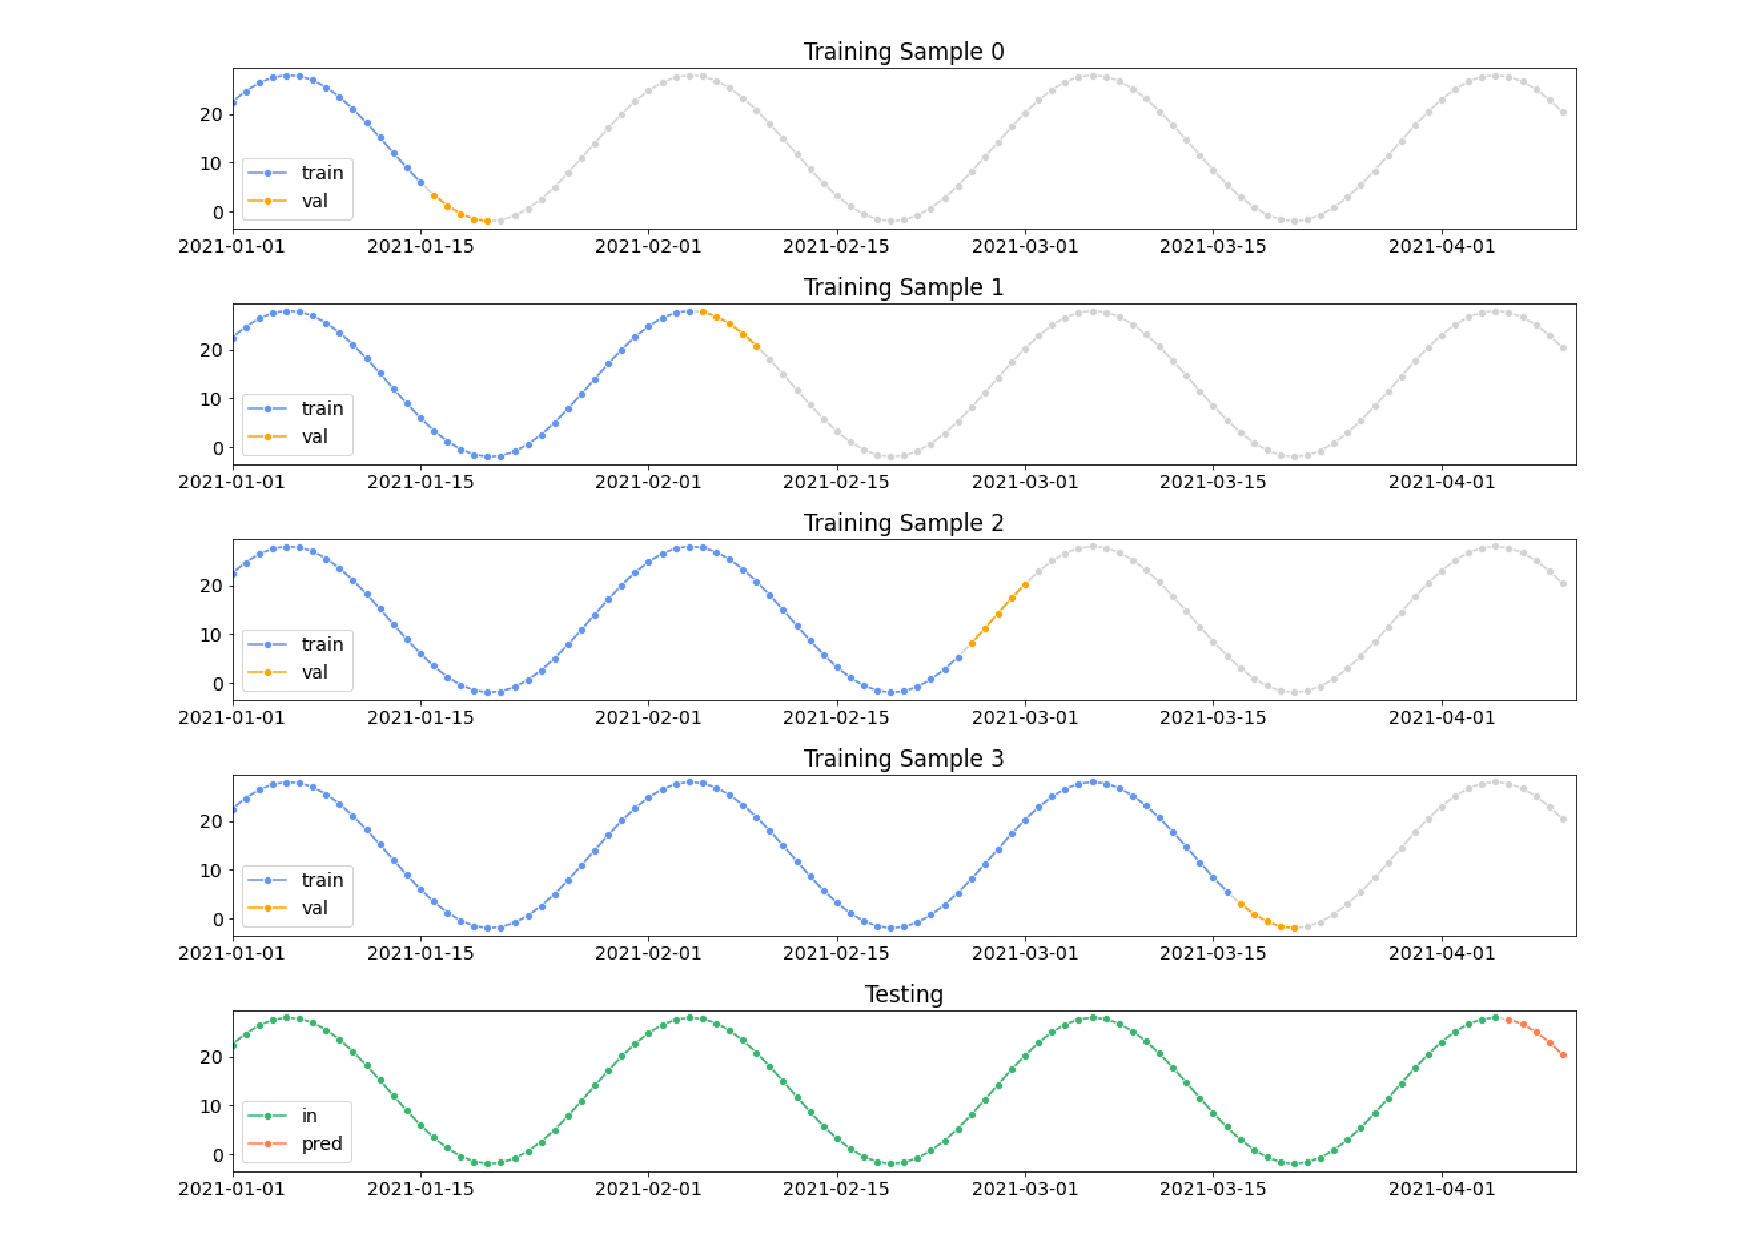
\includegraphics[width=\linewidth]{figures/expanding_window.pdf}
        \caption{Expanding window training samples illustration.}
        \label{fig:expanding_window}
    \end{subfigure}\hfill
    \begin{subfigure}[t]{0.48\linewidth}
        \centering
        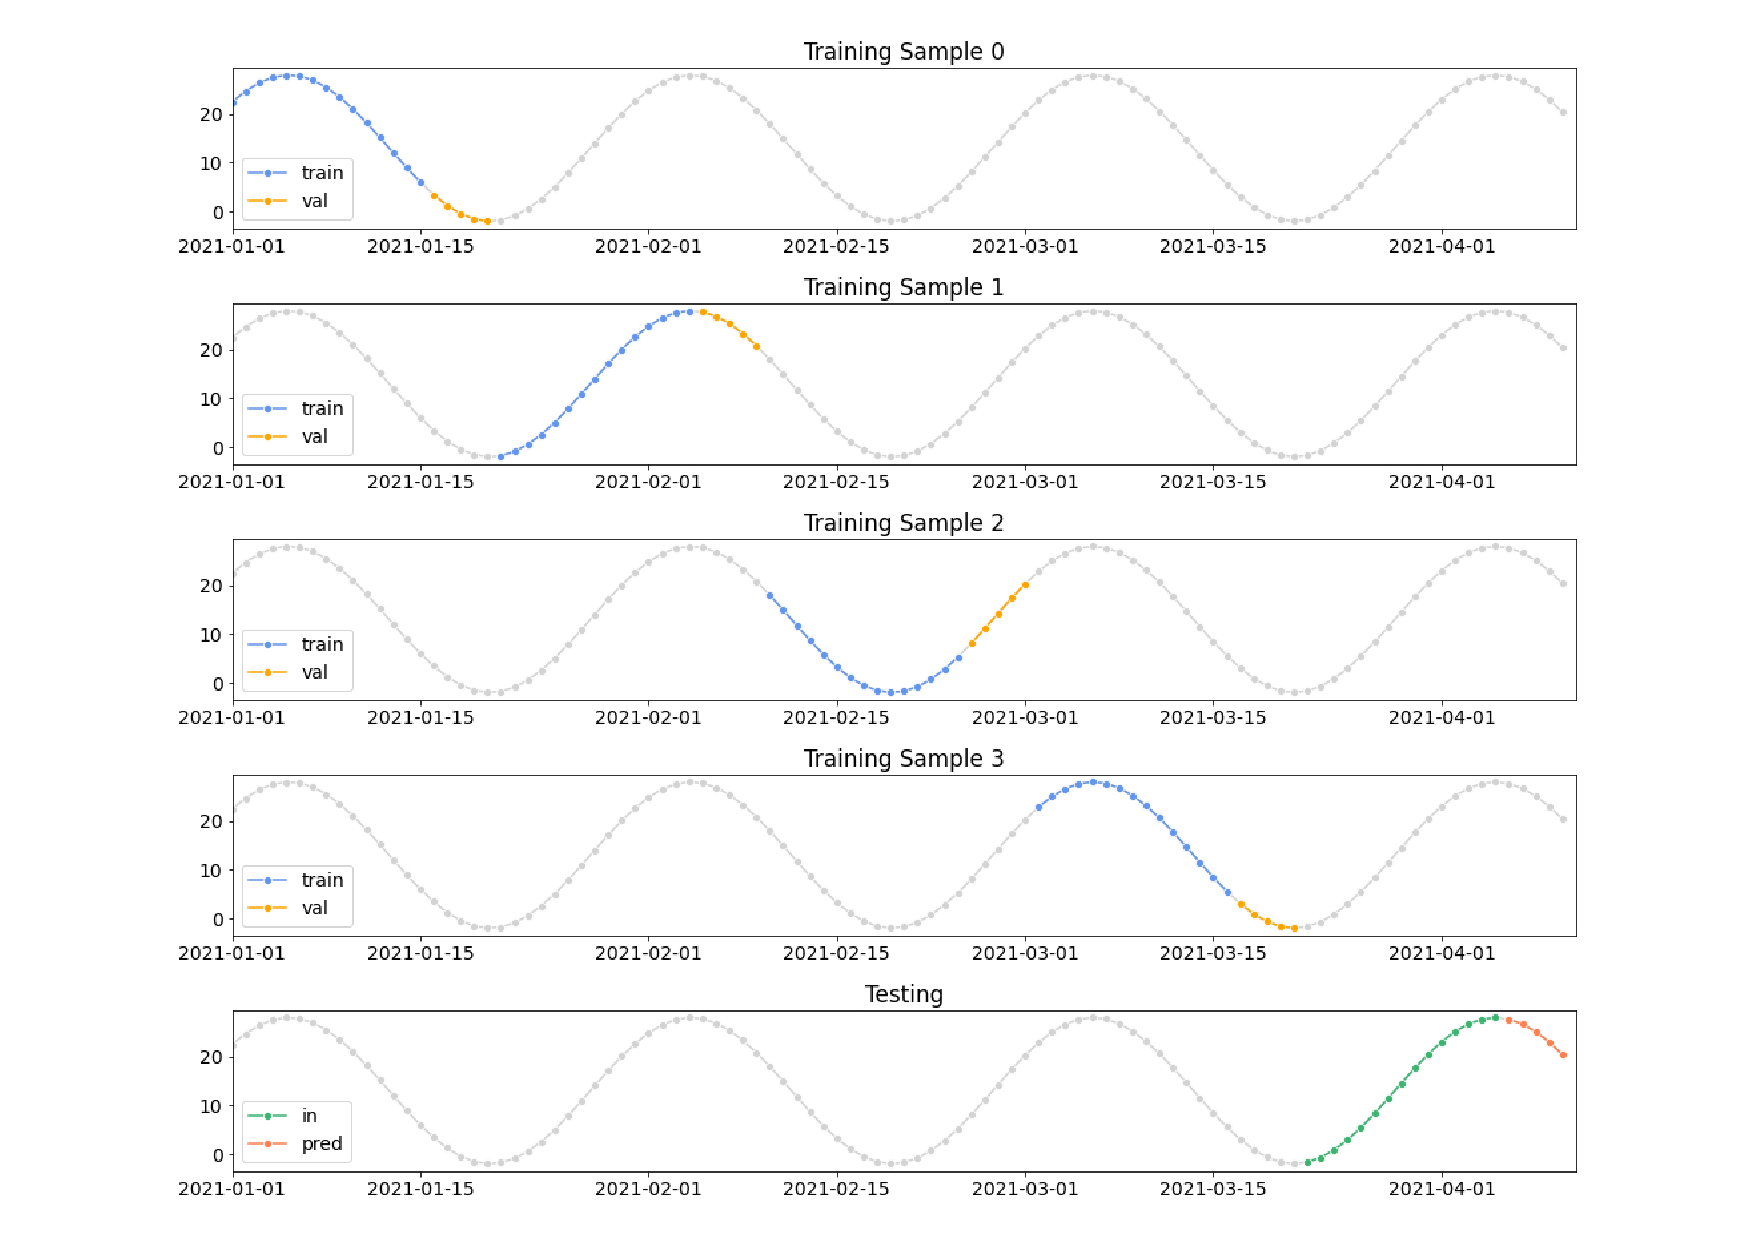
\includegraphics[width=\linewidth]{figures/sliding_window.pdf}
        \caption{Sliding window training samples illustration.}
        \label{fig:sliding_window}
    \end{subfigure}
    \caption{Windowing strategies used to generate training samples.}
    \label{fig:windowing_strategies}
\end{figure}